\chapter{Experiment Setup ~20}

\section{Jefferson Lab CEBAF}

The PRex and CREx experiments are conducted at the Continuous Electron Beam Accelerator Facility (CEBAF) housed within Jefferson Lab. Since its inception in the early 1990s, CEBAF has been a global pioneer, forging paths in nuclear physics research.

The heart of CEBAF is its linear accelerators (linacs), specifically the North and South linacs. These linacs serve as the key elements where electrons amass energy, essential for the facility's experimental proceedings.

Connecting these two linacs are the Recirculation Arcs, which are magnetic systems designed to curve the electron beam, redirecting it back into the linacs for additional energy enhancement during successive passes. An added function of the Recirculation Arcs is to facilitate the separation of electron beams of varying energy levels, post their multiple circulations through the linacs. This structural alignment and the operational interplay between the components ensure precision and efficacy in executing complex nuclear physics experiments like PRex and CRex.


% Para. 2
% \begin{itemize}
%     \item 12GeV upgrade
%     \item RF separator
%     \item RF cavities, cooled 
%     \item Beam energy and current ability
%     \item accelerated up to 5 times though both linacs, producing a nominal energy of 10.9GeV. 
%     \item 1497MhZ split into three 499MHz.
%     \item north and south linacs each can gen 1.1GeV 
%     \item East/West Arc bend the beam to accelerate again 
%     \item Hall ABC, 10.9GeV 
%     \item Hall D 12GeV
% \end{itemize}

The Jefferson Lab's CEBAF upgrade project, completed in 2014, introduced a number of significant enhancements. The modifications included the addition of five cryomodules to each Linac section, each housing 7-cell cavities capable of handling a higher RF field, courtesy of advanced surface treatments.

Each of these upgraded linacs can now facilitate an energy gain of 1.1 GeV, enabling the electron beam to achieve 2.2 GeV during each circulation. Post traversing the south linac, the electron beam can be partitioned into three distinct 499 MHz beams.

The facility's design allows for the electron beam to be accelerated up to five times through both linacs, producing a nominal energy output of 10.9 GeV. Experimental Halls A, B, and C each can receive a beam carrying energy that is one-fifth of the full 5-pass energy.

Additionally, the beam directed to Hall D can be re-accelerated in the north linac, reaching energy levels as high as 12 GeV. This upgrade has elevated the capacity and flexibility of the CEBAF, further enhancing its research potential.

% Para. 3
% \begin{itemize}
%     \item PRex requires high polarized beam 
%     \item high current to be able to get enough statistics to be able to measure 
%     \item PRex experiment choose CEBAF
%     \item high current
%     \item polarize beam ability
% \end{itemize}

The PRex-II and CREx experiments aim to quantify the thickness of the neutron skin by analyzing parity-violated asymmetry. To achieve a reliable measurement with a sufficient confidence interval, a significant volume of statistical data is required. This necessity is met by the capabilities of CEBAF, which can generate a polarized electron beam with a current reaching up to $200 uA$ and a polarization level in the range of $80-90\%$. Such robust performance plays a pivotal role in enabling the execution and success of the PRex and CREx experiments.


\begin{figure}
     \centering
     \begin{subfigure}[b]{0.45\textwidth}
         \centering
         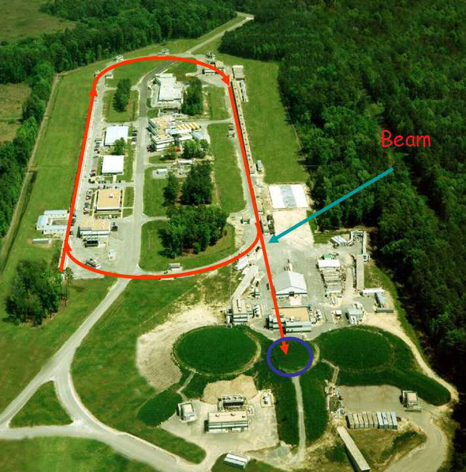
\includegraphics[width=\textwidth]{images/chap3/JLab_cebaf_photo.png}
         \caption{Photo of CEBAF}
         \label{Photo of CEBAF}
     \end{subfigure}
     \hfill
     \begin{subfigure}[b]{0.45\textwidth}
         \centering
         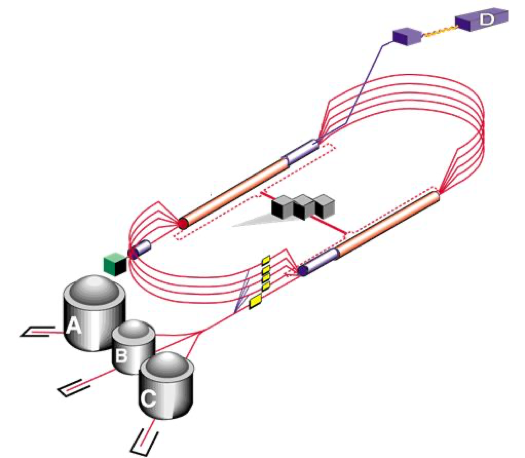
\includegraphics[width=\textwidth]{images/chap3/JLab_cebaf.png}
         \caption{JLAB CEBAF}
         \label{JLAB CEBAF}
     \end{subfigure}
\end{figure}

\section{Beam injection}



\begin{figure}
    \centering
    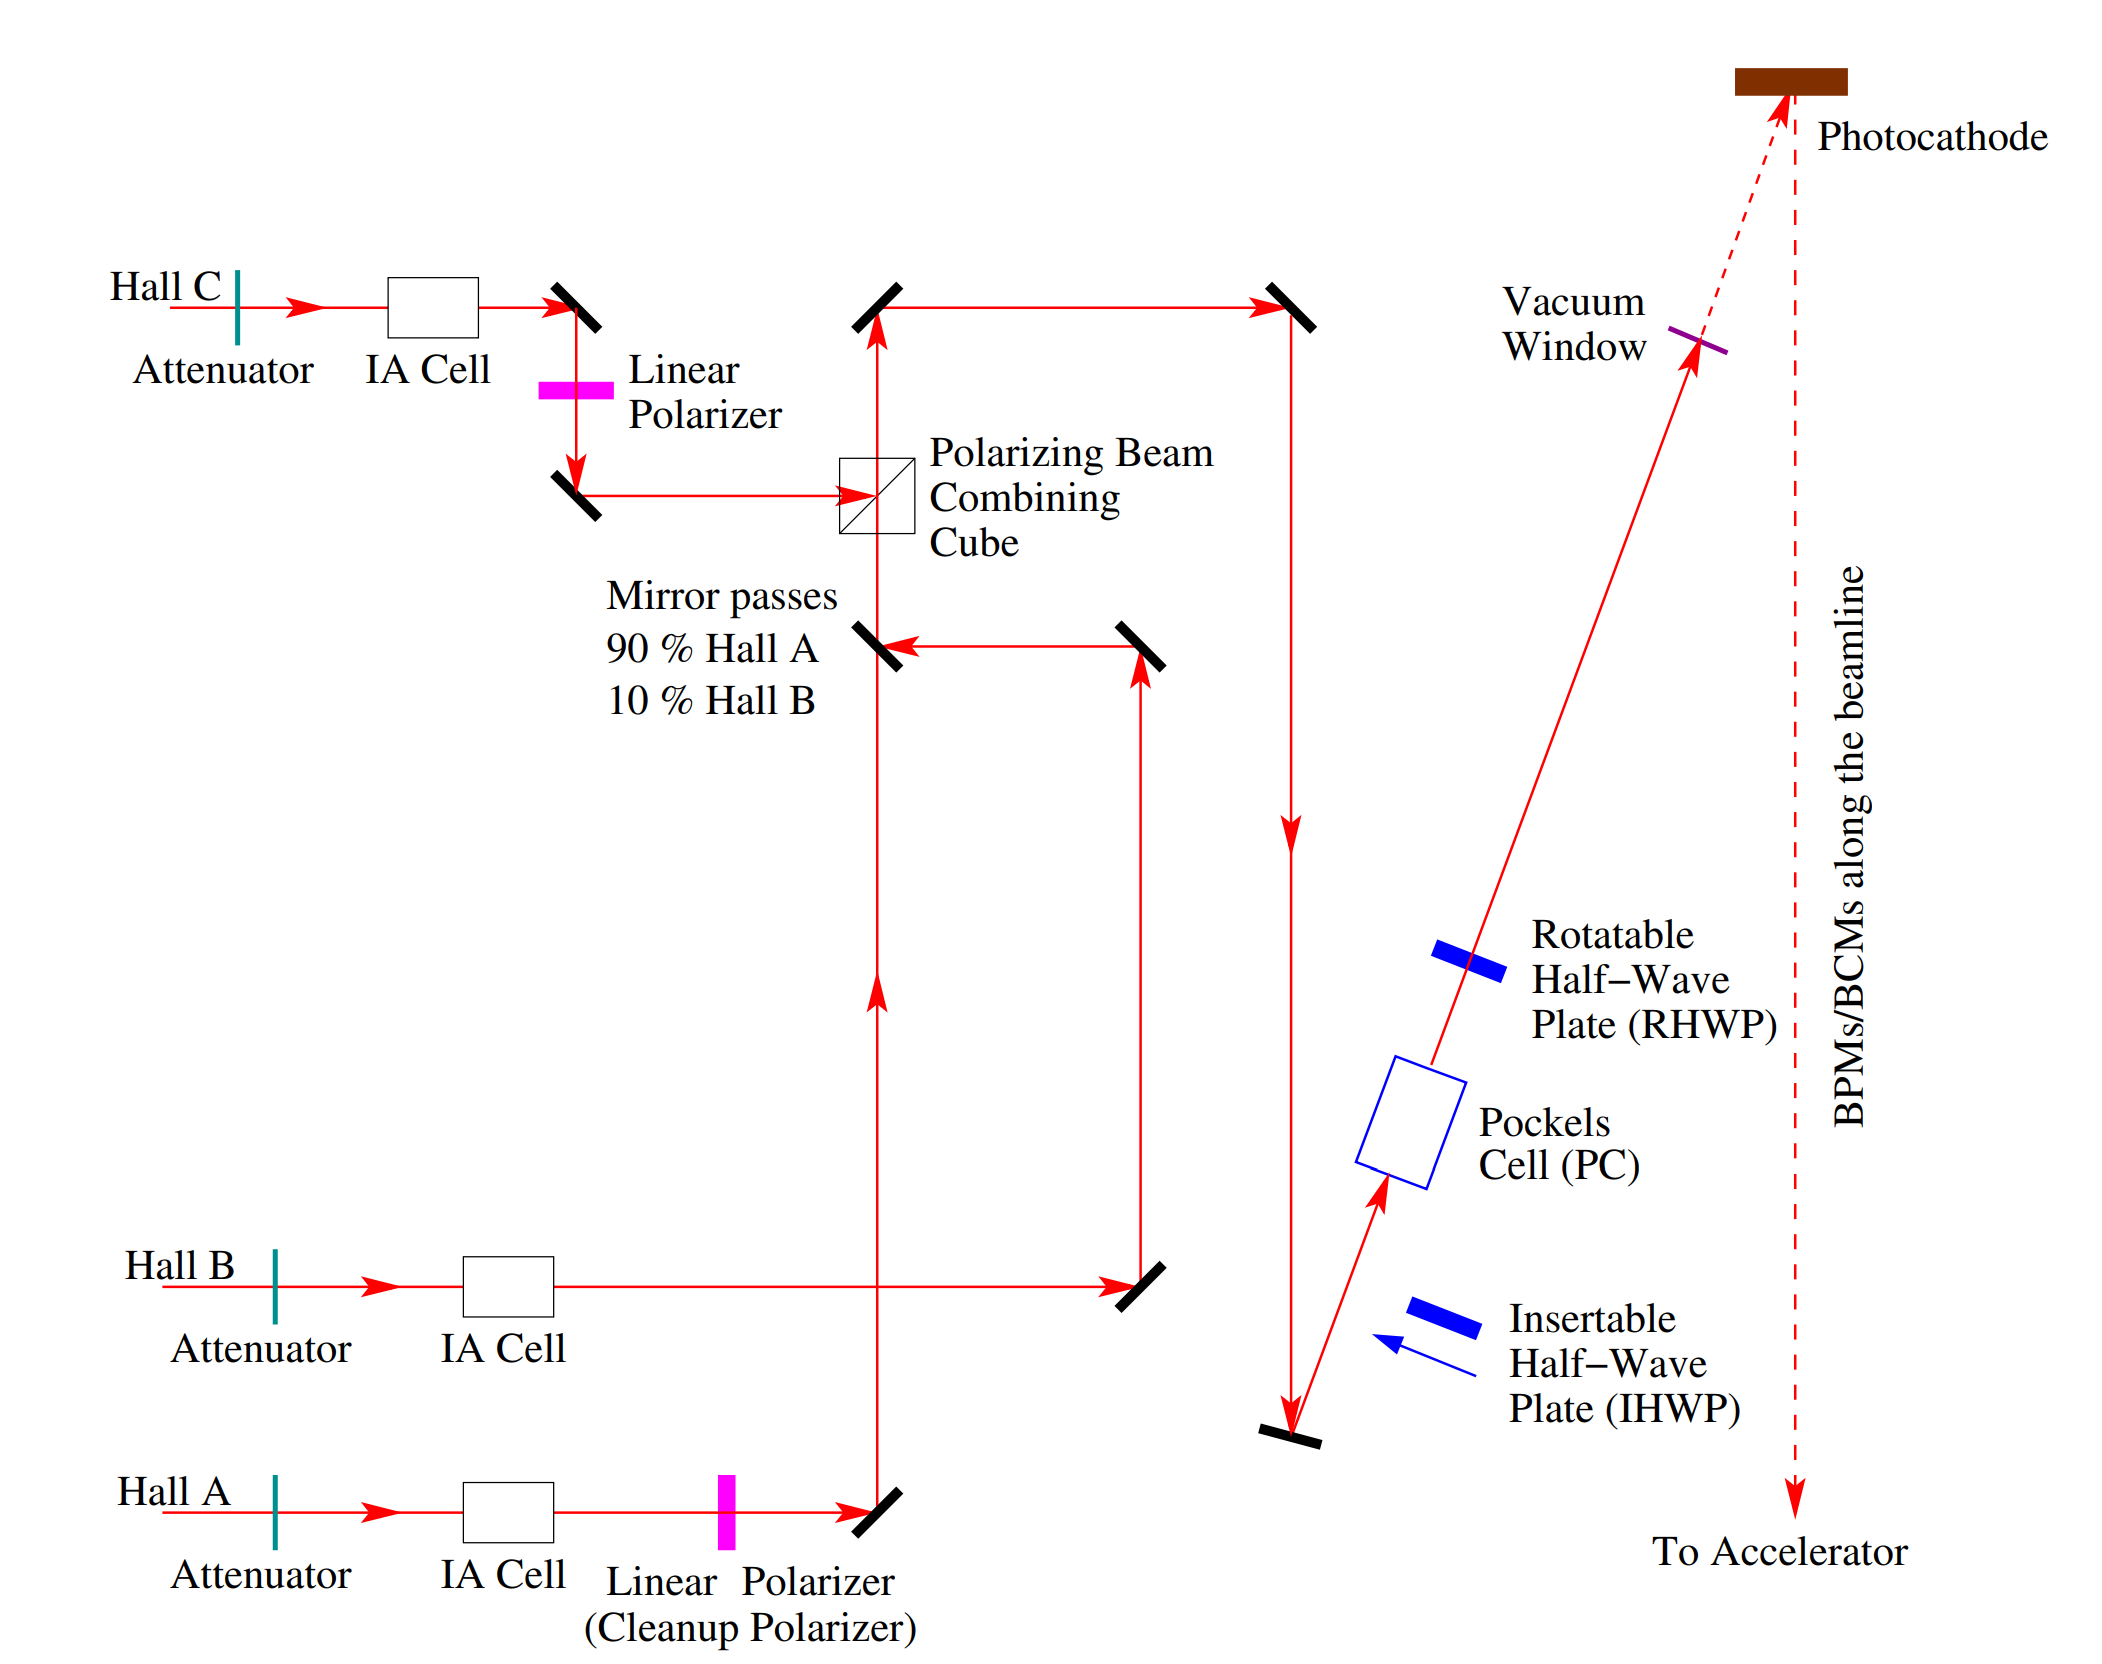
\includegraphics[width=\textwidth]{images/chap3/jlab_polarized_source.png}
    \caption{Caption}
    \label{fig:enter-label}
\end{figure}
\subsection{Polarized Beam}

\subsection{Helicity Control}

\section{Beam monitor}
\subsection{Polorimeter}
\subsection{Compton}
\subsection{Beam Position Monitor}
\subsection{Beam current monitor}

\section{Target System}


\begin{itemize}
    \item target chamber
    \item target ladder 
    \item different target type and its usage
\end{itemize}

\section{High Resolution Spectrometer}

[intro]

\begin{itemize}
    \item core part of the Hall A 
    \item magnet package
    \item septum magnet
    \item tracking detector (VDC, GEM)
    \item AT
    \item trigger
\end{itemize}

\subsection{Sieve plane}

\begin{itemize}
    \item provides the ground truth dataset for the calibration. (Regression model)
    \item CAD structure of the sieve 
    \item location of the sieve. sieve in / out
    \item merge some of the plot from next chamber
    \item  will give a detailed introduction of how to leverage the sieve to calibrate the spectrometer
\end{itemize}

\subsection{Magnet Chain of the HRS}
\subsubsection{Septum Magnet}
\subsubsection{QQDQ magnet package}
\subsection{Vertical Drift Chamber}

\begin{itemize}
    \item GEM foil
    \item GEM foil structure, microscope image
    \item GEM foil magnetic field simulation (Garfield simulation)
\end{itemize}


\begin{itemize}
    \item GEM detector structure
    \item AI window used de-polarized the window
    \item Window 
    \item 3 GEM layers
    \item Read out strips 
    \item backbone 
    \item back chamber used for balance the pressure, prevent the readout board bend
\end{itemize}


\begin{itemize}
    \item How GEM works
    \item Garfild simulation 
\end{itemize}

\subsection{GEM detector}
\subsection{HV}

\begin{itemize}
    \item High Voltage Regestor chain 
    \item HV models 
    \item High Voltage Scan
    \item the lowest voltage that meets the requirements
\end{itemize}

\subsection{LV}

\begin{itemize}
    \item The Low voltage power supply
    \item current consideration 
    \item images of the low voltage
    \item cooling 
\end{itemize}

\subsection{Gas Flow}

    \begin{itemize}
        \item The Gas flow system
        \item bubbler
        \item how to distribute to the chamber 
        \item gas flow in the chamber
    \end{itemize}

\subsection{DAQ system of the GEM detector}

\subsubsection{APV}
\begin{itemize}
    \item APV 25, charge sensitive pre-amplifier
    \item HDMI cable
    \item Noise Reduction technics (the fifth channel of the HDMI is not good)
\end{itemize}

\subsubsection{MPD}

\begin{itemize}
    \item analog to digital converter
    \item CPU 
    \item event rate limitations
\end{itemize}



\subsection{QUATZ / AT}
\subsection{trigger system}

